\chapter{Implementation And Testing}

	\section{The architecture the software}
	As in chapter \ref{chDesign}, in this section class diagrams are used in order to clarify the description. Again, such description follows a top-down approach: section \ref{impl_arch} gives an overview of the architecture and for this reason the diagram in figure \ref{fig:implementation_names} contains only the names of the classes. The following sections study in deep specific aspects of the software and, consequently, contain more detailed diagrams.


		\subsection{Overview}\label{impl_arch}
		Figure \ref{fig:implementation_names} shows the class diagram of the whole software. 
		According to the design specifications defined in chapter \ref{chDesign}, the software is organized in four main parts, each of which has its own role.

		\begin{figure}[h]
		  \begin{center} 
		    \fbox{	
		       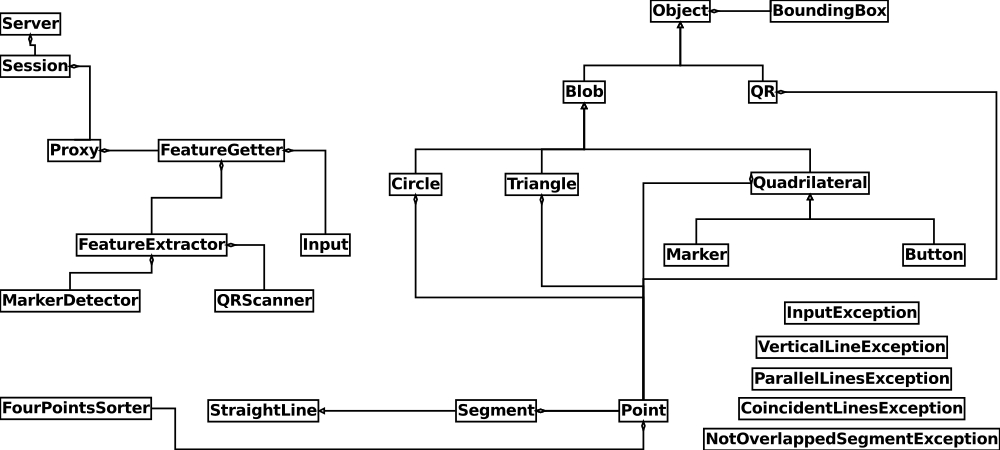
\includegraphics[width=\textwidth*\real{0.9}]{images/ch_06/implementazione_solo_nomi.jpg}
		    }
		  \end{center} 
		  \caption{\textit{Class diagram which illustrates the whole architecture of the software}}  
		  \label{fig:implementation_names}
	 	\end{figure}
 
		Classes \emph{Server} and \emph{Session} manage the communication with \mbox{ACT-R}, implemented by a client server approach.
		Classes \emph{Proxy}, \emph{FeatureGetter}, \emph{Input}, \emph{FeatureExtractor}, \emph{MarkerDetector} and \emph{QRScanner} have the role of extracting the feature from the input data and preparing the messages to be sent to the cognitive architecture.
		\emph{Object}, \emph{BoundingBox}, \emph{Blob}, \emph{QR}, \emph{Circle}, \emph{Triangle}, \emph{Quadrilateral}, \emph{Marker} and \emph{Button} form the object hierarchy.
		\emph{InputException}, \emph{NotOverlappedSegmentException}, \emph{ParallelLinesException}, \emph{VerticalLineException}, \emph{CoincidentLinesException}, \emph{FourPointsSorter}, \emph{StraightLine}, \emph{Segment} and \emph{Point} represent the utility classes.
	
		Comparing the classes shown in figure \ref{fig:implementation_names} with the design choices defined in chapter \ref{chDesign}, the reader can notice two facts: both the feature extractor and the class hierarchy parts strictly adhere to the project and, accordingly to the design choices, the classes containing the utility functions and the features for the communication with \mbox{ACT-R} have been properly developed.
		%The following sections presents the implementation of the whole classes, focusing mainly on these two latter parts of the software. 

	
		\subsection{Communication with ACT-R}
		The part responsible for the communication with the cognitive architecture is composed by the classes \emph{Server} and \emph{Session}. \todo{}

\newpage
		\subsection{Feature Extraction}
		Image \ref{fig:impl_feat_extraction} shows a class diagram of the implementation of the feature extractor part of the software. 
		Analyzing it, the reader can notice that the implementation adheres very good to the design specifications, described at page \pageref{featExtraction}. 
		The classes, in fact, are the same but with more attributes and methods. 
		Such additions have been introduced at development time, as the requirements became clearer.
		Notice that some methods, like for example \emph{setCroppedImage} in FeatureExtractor class, are used to obtain goals different from the one described in this work, but make sense in the general context of the team work. This topic is better explained in the introductory part of chapter \ref{chDesign}. 

		\begin{figure}[h]
		  \begin{center} 
		    \fbox{	
		       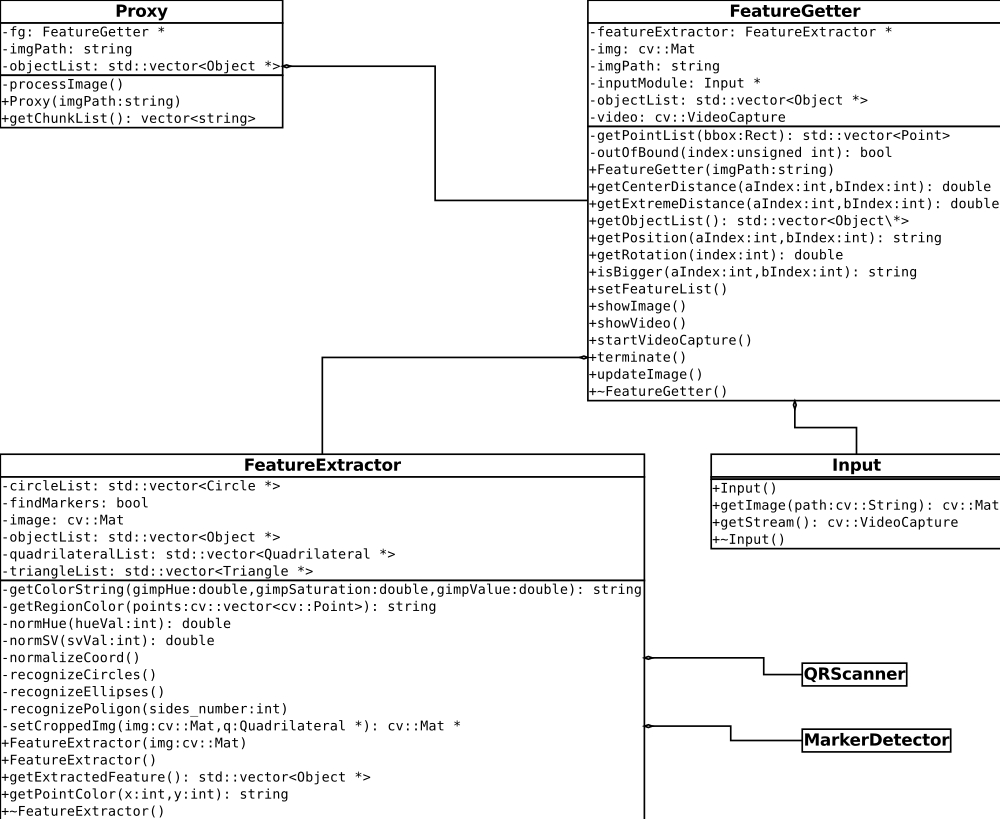
\includegraphics[width=\textwidth*\real{0.9}]{images/ch_06/fe.jpg}
		    }
		  \end{center} 
		  \caption{\textit{Class diagram describing the implementation of the feature extraction part of the software}}  
		  \label{fig:impl_feat_extraction}
	 	\end{figure}	


		\subsection{Object Hierarchy}
		As it can be noticed comparing the diagram in figure \ref{fig:impl_hierarchy} with the diagram of the design at page \pageref{fig:HierarchyDesign}, the differences between the implementation and the project are minimal. 
		In fact, further classes have not been introduced; rather, the existing ones have been provided with additional parameters and methods, as for example, the attributes \emph{color} and \emph{center}.
		According to the iterative development process, different parameters have been added at different moments of the development.
		\begin{figure}[h]
		  \begin{center} 
		    \fbox{	
		       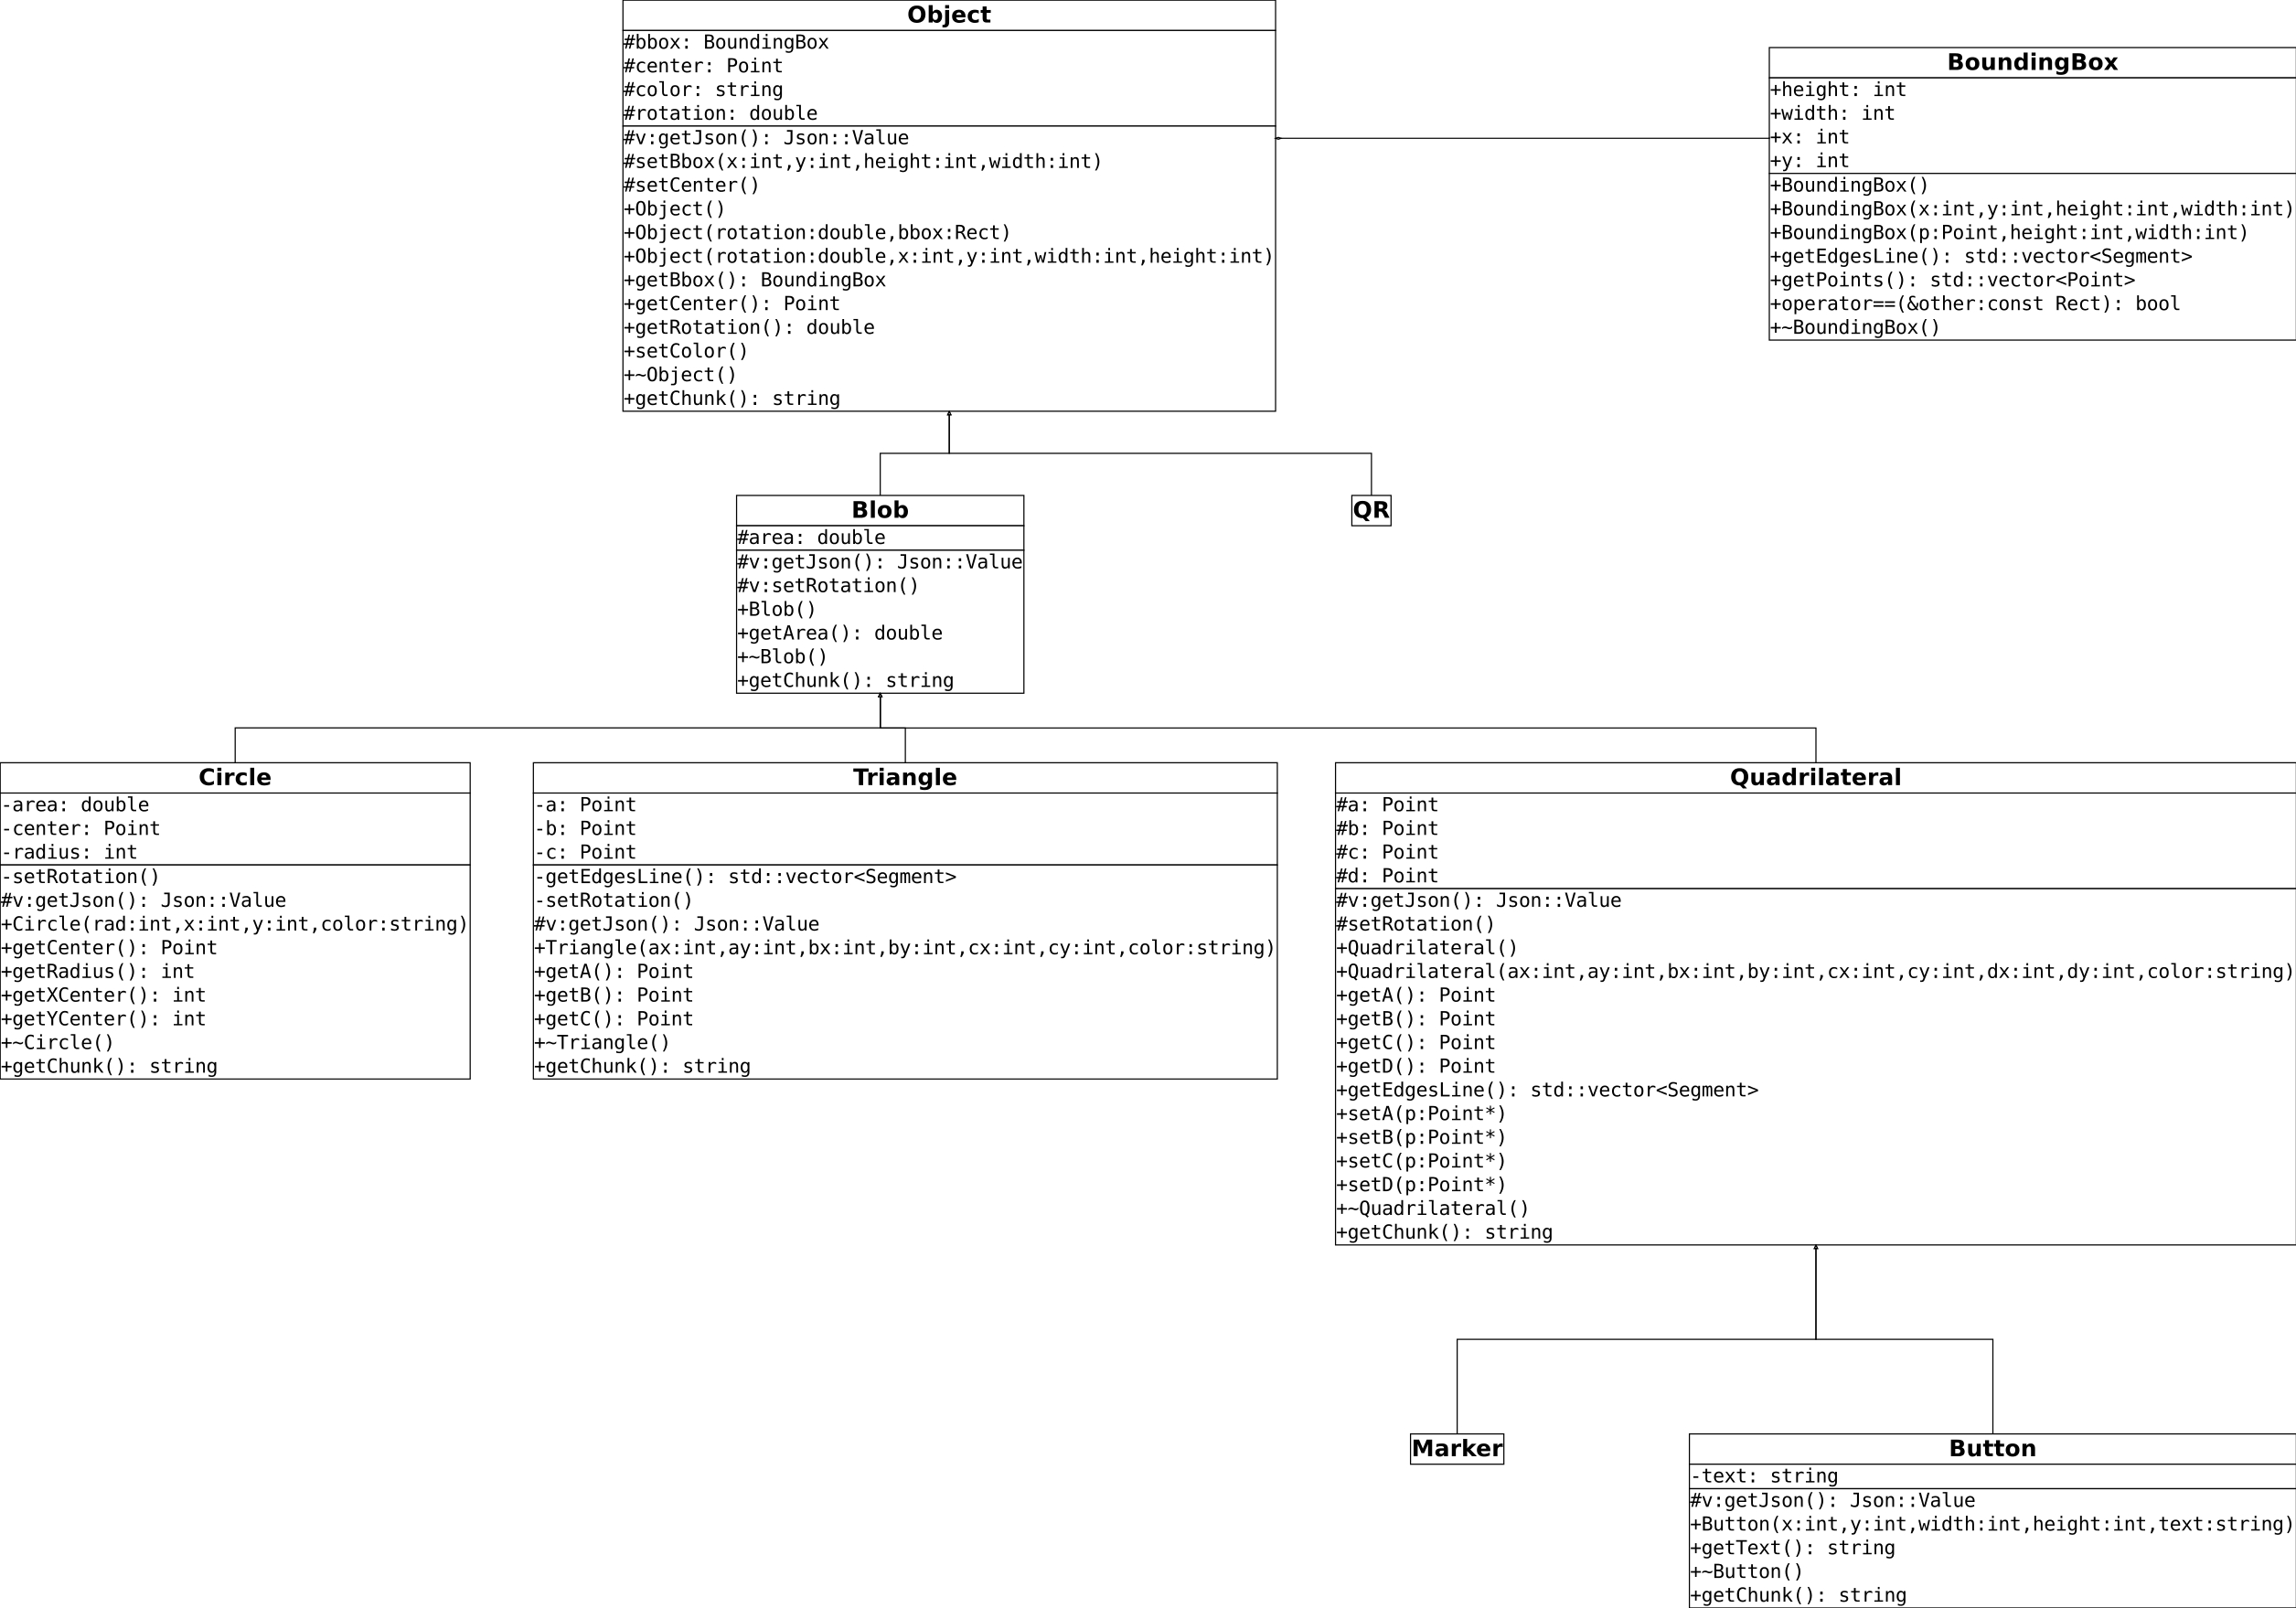
\includegraphics[width=\textwidth*\real{0.9}]{images/ch_06/hierarchy.jpg}
		    }
		  \end{center} 
		  \caption{\textit{Class diagram that shows the implementation of the object hierarchy}}  
		  \label{fig:impl_hierarchy}
	 	\end{figure}

	

		\subsection{Utility Part}
		The utility part is composed by the classes \emph{InputException}, \emph{NotOverlappedSegmentException}, \emph{ParallelLinesException}, \emph{VerticalLineException}, \emph{CoincidentLinesException}, \emph{FourPointsSorter}, \emph{StraightLine}, \emph{Segment}, \emph{Point} and another module containing functions. The latter, as it is not a class, is not included in the diagram in figure \ref{}. 

		\emph{InputException}, \emph{NotOverlappedSegmentException}, \emph{ParallelLinesException}, \emph{VerticalLineException} and \emph{CoincidentLinesException} are exceptions classes, used to handle all the anomalous or exceptional events occurring during the execution of the software. 

		\emph{StraightLine}, \emph{Segment} and \emph{Point} represent geometrical entities. Such elements are fundamental structures for creating the objects in the hierarchy and making evaluations between couples of objects.
		Such evaluations can be both qualitative and quantitative, as, for example, the distances between the centers of two objects or the relative positions of one object in respect with another.

		\emph{FourPointsSorter} and the function module contain the basic methods which are fundamental for all the operations executed by all the other classes of the software.

	

	%\clearpage
 	%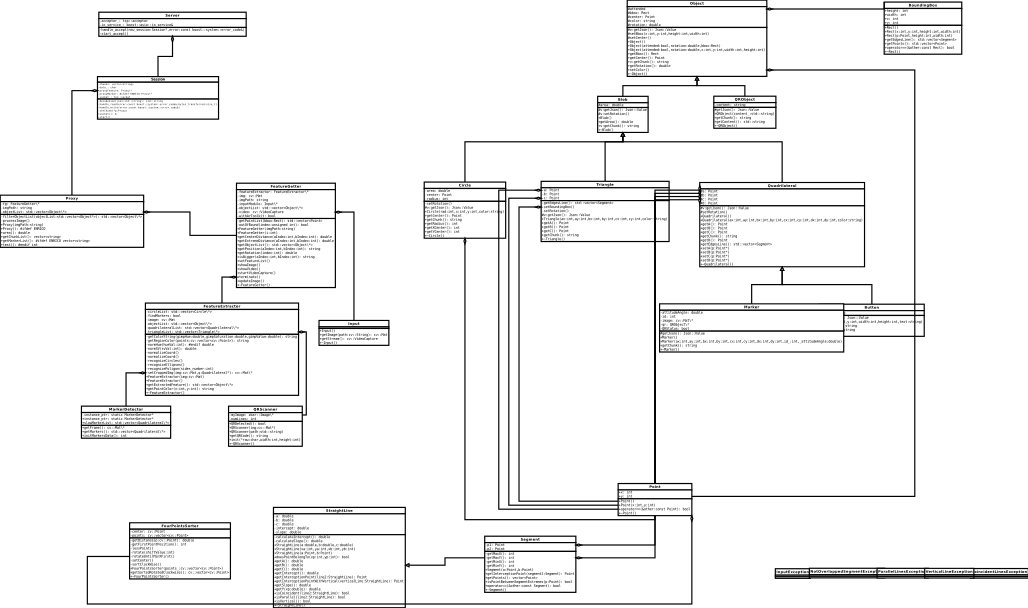
\includegraphics[angle=90,height=\textheight]{images/ch_06/implementation.jpg}\thispagestyle{empty}
\begin{comment}
	\pagestyle{empty}
	\begin{center} 	
	\fbox{	
		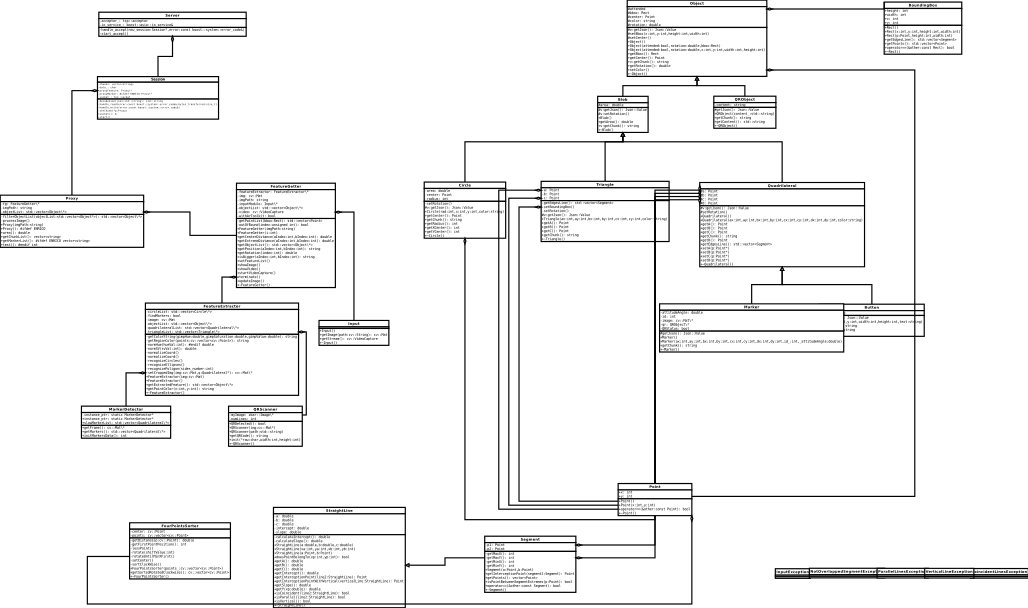
\includegraphics[angle=90,height=26cm]{images/ch_06/implementation.jpg}%\thispagestyle{empty}
	}
	%\caption{\textit{Class diagram illustrating a high level overview of the implementation}} 
	\label{fig:impl}
	\end{center}
\end{comment}	


 
	\section{Testing}
\begin{comment}

	As it can be seen in the picture, the software is logically divided in the four main components introduced in the design chapter (see \ref{chDesign}).
%, respecting the in the design specifics described in chapter \ref{chDesign}. 
	Both the feature extraction part and the class hierarchy respect the design specifications, described in such chapter. The classes responsible for the communication with \mbox{ACT-R} and the utility part.
The communication with  and


	\newpage
	
	\begin{sidewaysfigure}[hbtp]
	   \thispagestyle{empty}	
 	   \centering
	   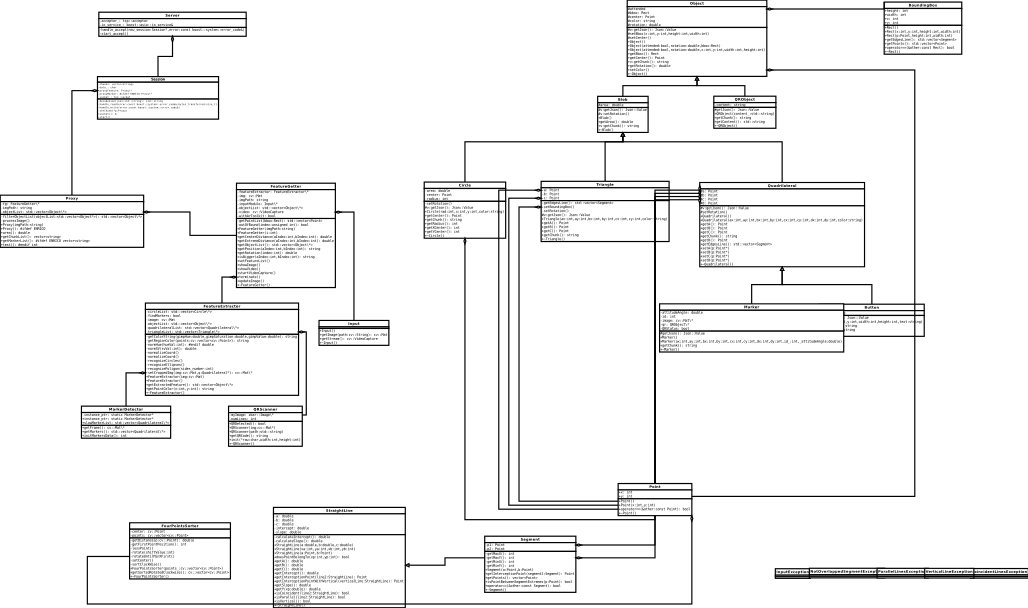
\includegraphics[height=\textheight]{images/ch_06/implementation.jpg}
	   
	  \caption{\textit{Class diagram illustrating the class hierarchy of the recognized objects}}  
	  \label{fig:HierarchyDesign}
 	\end{sidewaysfigure}

\newpage

\relax
	\AddToShipoutPicture*{ \\ \relax
	  \setlength{\unitlength}{1mm} 
	  \put(<10>, <10>){  
	    \makebox(0,0){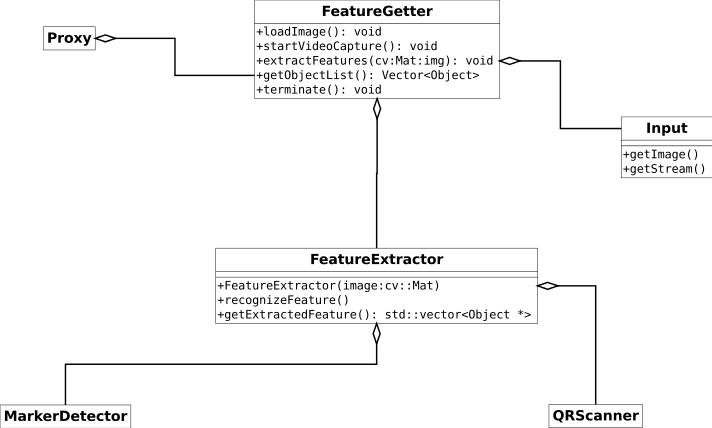
\includegraphics{images/ch_05/feature.png}}}} 
	ciao

	
\end{comment}

	%\section{COmmunication with ACT-R}
	%ciao
